%==================== TITLE SLIDE ====================
{
\setbeamertemplate{footline}{}
\begin{frame}[noframenumbering]

\vspace{2cm}

\begin{center}
    {\fontsize{24}{28}\selectfont \color{tugreen}
    Case Study II: \\[0.3cm]
    Styrian Health Data}
\end{center}

\vspace{1.25cm}

\begin{flushleft}
    {\large \color{black}
    Rohith B Chowdappa\\
    Sandra A Shaji\\
    Nixon M Paulson\\
    Maria Cherian}
\end{flushleft}

\end{frame}
}

\begin{frame}

    \vspace{0.5cm}

    {\raggedright
        {\fontsize{16}{20}\selectfont \color{tugreen} Random Forest and Selected Hypotheses}
    }
    \vspace{0.5cm}
    {
    \setbeamercolor{item}{fg=tugreen}
    \begin{itemize}
        \item Applied \textbf{Random Forest} to analyze blood pressure
            \begin{itemize}
                \item H1: Can we statistically prove the relationship between age and BP?
                \item H2: Are there differences in blood pressure by gender, diabetes, smoking, cholesterol, well-being?
            \end{itemize}
    \end{itemize}

    }

\end{frame}

\begin{frame}

    \vspace{0.5cm}

    {\raggedright
        {\fontsize{16}{20}\selectfont \color{tugreen} Final Dataset }
    }
    \vspace{0.5cm}
    {
    \setbeamercolor{item}{fg=tugreen}
    \begin{itemize}
        \item \textbf{Original rows:} 16,386
        \item \textbf{Rows after removing nulls:} 16,004  (removed 382)
        \item \textbf{Rows after filtering age 13--100:} 15,219  (removed 785)
        \item \textbf{Total removed:} 1,167
    \end{itemize}

    }

\end{frame}

\begin{frame}

    \vspace{0.5cm}

    {\raggedright
        {\fontsize{16}{20}\selectfont \color{tugreen} Data Preparation for Random Forest}
    }
    \vspace{0.5cm}
    {
    \setbeamercolor{item}{fg=tugreen}
    \begin{itemize}
        \item Random Forest requires all input features to be numeric
            \begin{itemize}
                \item Converted categorical/boolean columns to integers
            \end{itemize}
    \end{itemize}

    }

\end{frame}

\begin{frame}
    \vspace{0.5cm}
    {\raggedright
        {\fontsize{16}{20}\selectfont \color{tugreen} Random Forest — Blood Pressure Prediction}
    }
    \vspace{0.5cm}
    {
    \setbeamercolor{item}{fg=tugreen}
    \begin{itemize}
        \item Multi-output Random Forest model to predict \textbf{Systolic and Diastolic BP}
        \item \textbf{Features used:} Age, Gender, Smoker, Known Blood Sugar, Known Cholesterol, Under Treatment, Health Condition
        \item \textbf{Hyperparameters:}
        \begin{itemize}
            \item n\_estimators=500, max\_features='sqrt'
            \item min\_samples\_leaf=5, max\_depth=None
            \item random\_state=42, n\_jobs=-1
        \end{itemize}
    \end{itemize}
    }
\end{frame}

%==================== Actual vs Predicted Slide ====================
\begin{frame}{}
    \vspace{0.5cm}
    {\raggedright
        {\fontsize{16}{20}\selectfont \color{tugreen} Random Forest — Model Evaluation}
    }
    \centering
    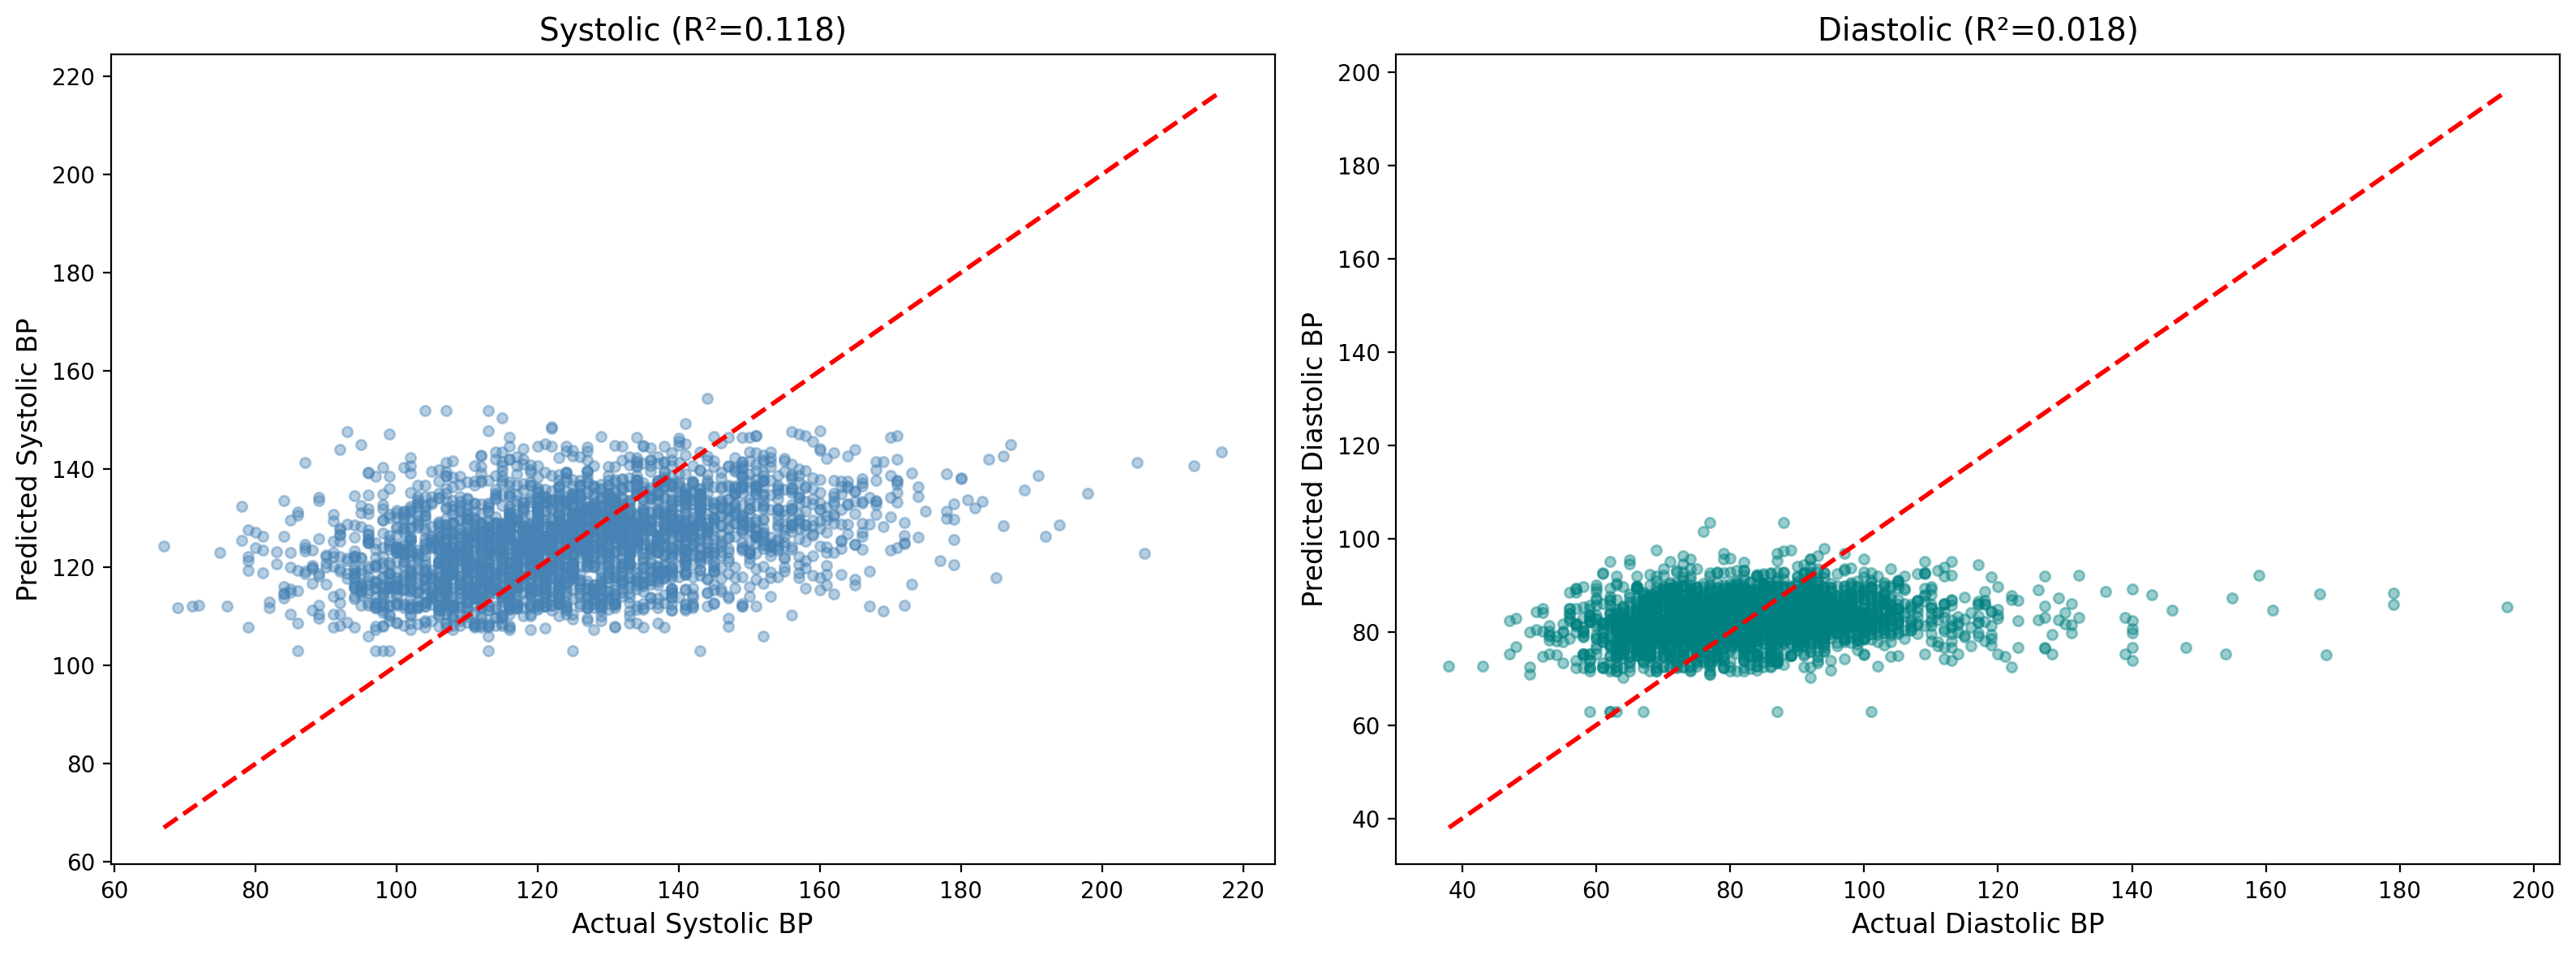
\includegraphics[height=0.6\textheight]{../presentation/figures/bp_actual_vs_predicted_fig.png}

    \vspace{0.3cm}
    \begin{itemize}
        \item Systolic BP predictions follow a weak positive trend
        \item Diastolic BP predictions are very noisy
    \end{itemize}
\end{frame}

\begin{frame}{}
    \vspace{0.5cm}
    {\raggedright
        {\fontsize{16}{20}\selectfont \color{tugreen} Random Forest — Model Evaluation}
    }
    \vspace{0.5cm}
    {
    \setbeamercolor{item}{fg=tugreen}
    \begin{itemize}
        \item \textbf{Systolic BP:}
        \begin{itemize}
            \item R² = 0.118 — low, model explains only 12\% of variance
            \item MAE = 14.05 mmHg, RMSE = 17.98 mmHg
        \end{itemize}
        \item \textbf{Diastolic BP:}
        \begin{itemize}
            \item R² = 0.018 — almost no predictive power
            \item MAE = 10.70 mmHg, RMSE = 14.43 mmHg
        \end{itemize}
        \item Observations:
        \begin{itemize}
            \item Overall model fit is weak — variance in BP is high
            \item RMSE $>$ MAE indicates presence of outlier predictions
        \end{itemize}
    \end{itemize}
    }
\end{frame}

%==================== Feature Importance Slide ====================
\begin{frame}{}
    \vspace{0.5cm}
    {\raggedright
        {\fontsize{16}{20}\selectfont \color{tugreen} Feature Importance — BP Levels}
    }
    \vspace{0.3cm}
    \centering
    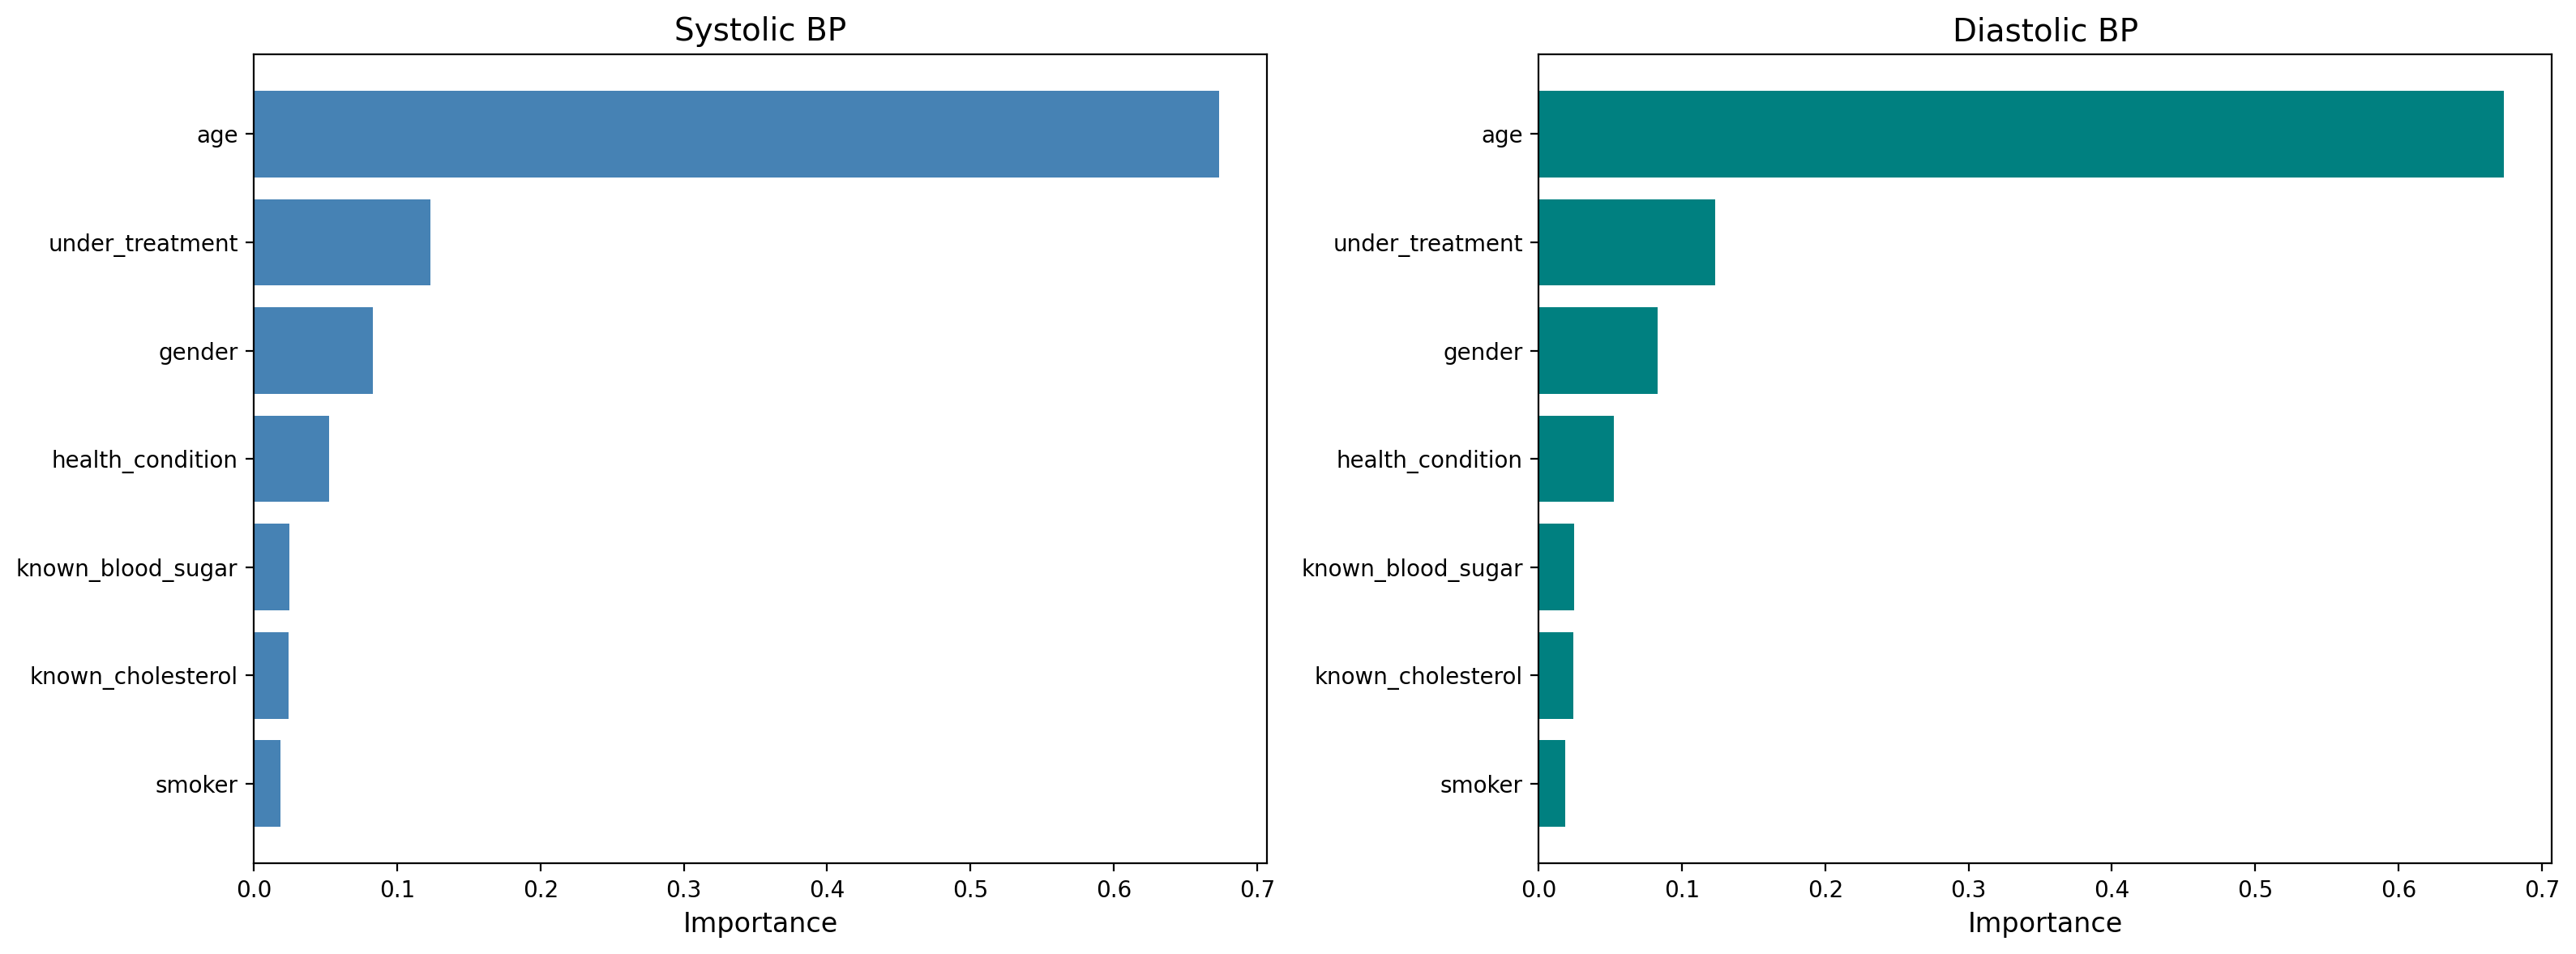
\includegraphics[width=0.99\textwidth,height=0.7\textheight]{../presentation/figures/bp_feature_importance_fig.png}
\end{frame}

\begin{frame}{}
    \vspace{0.5cm}
    {\raggedright
        {\fontsize{16}{20}\selectfont \color{tugreen} Feature Importance — BP Levels}
    }
    \vspace{0.5cm}
    {
    \setbeamercolor{item}{fg=tugreen}
    \begin{itemize}
        \item \textbf{Age} is the dominant feature in both models (importance $\approx$ 0.67)
        \item Followed by \textbf{Under Treatment}, \textbf{Gender}, and \textbf{Health Condition}
        \item Smoker, Blood Sugar, and Cholesterol contribute least
    \end{itemize}
    }
\end{frame}

\begin{frame}{}
    \vspace{0.5cm}
    {\raggedright
        {\fontsize{16}{20}\selectfont \color{tugreen} Overall Model Performance}
    }
    \vspace{0.5cm}
    {
    \setbeamercolor{item}{fg=tugreen}
    \begin{itemize}
        \item Model has \textbf{weak predictive power} for both BP types
        \item \textbf{Age} alone explains most of what the model can predict
        \item High MAE suggests predictions can be off by \textbf{10--14 mmHg} on average
        \item This is clinically significant — a 14 mmHg error matters in practice
    \end{itemize}
    }
\end{frame}

%==================== Diastolic-Only Model ====================
\begin{frame}{}
    \vspace{0.5cm}
    {\raggedright
        {\fontsize{16}{20}\selectfont \color{tugreen} Diastolic BP — Single Output Model}
    }
    \vspace{0.3cm}
    \centering
    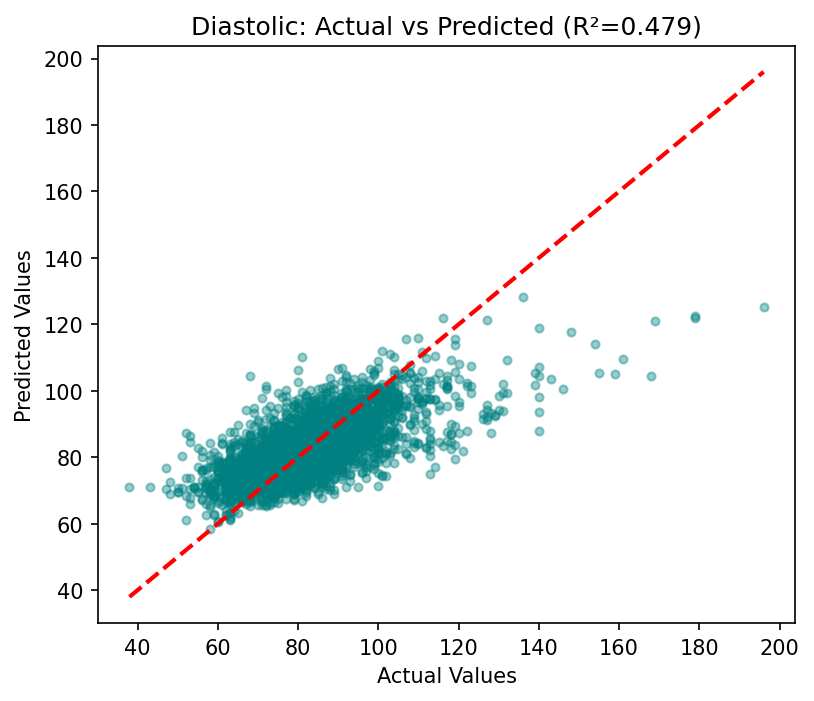
\includegraphics[width=0.48\textwidth]{../presentation/figures/bp_dia_prediction_fig.png}
    \hspace{0.01\textwidth}
    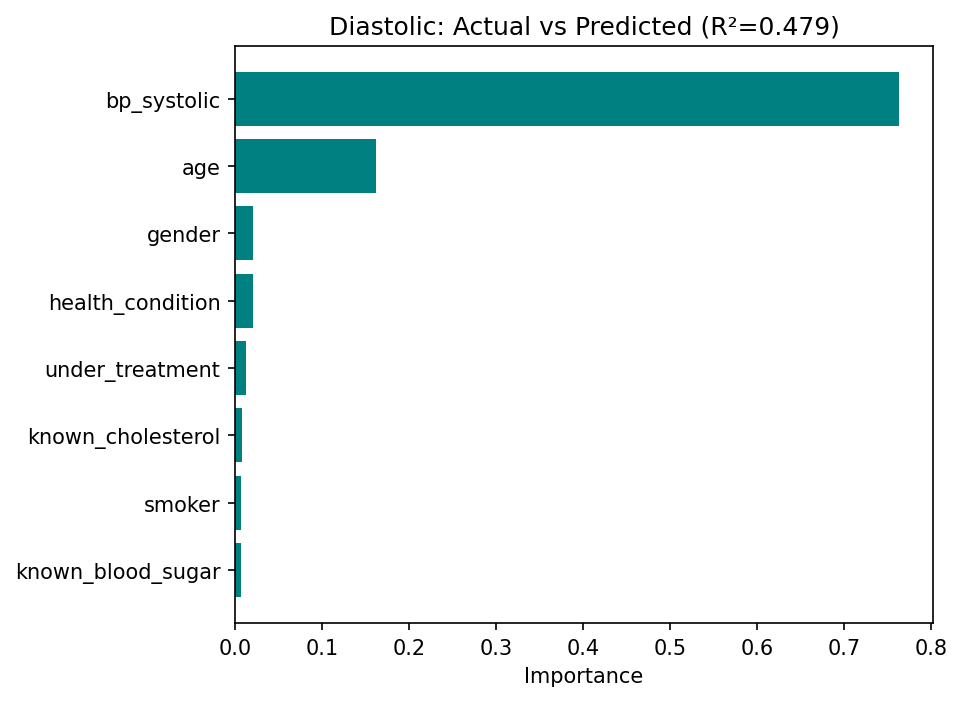
\includegraphics[width=0.48\textwidth]{../presentation/figures/bp_dia_featimp_fig.png}

    \vspace{0.3cm}
    {
    \setbeamercolor{item}{fg=tugreen}
    \begin{itemize}
        \item R² = 0.479, MAE = 7.73 mmHg, RMSE = 10.52 mmHg
        \item \textbf{Systolic BP} dominates as the strongest predictor (0.76)
        \item Age follows as second most important feature (0.16)
    \end{itemize}
    }
\end{frame}

%==================== Systolic-Only Model ====================
\begin{frame}{}
    \vspace{0.5cm}
    {\raggedright
        {\fontsize{16}{20}\selectfont \color{tugreen} Systolic BP — Single Output Model}
    }
    \vspace{0.3cm}
    \centering
    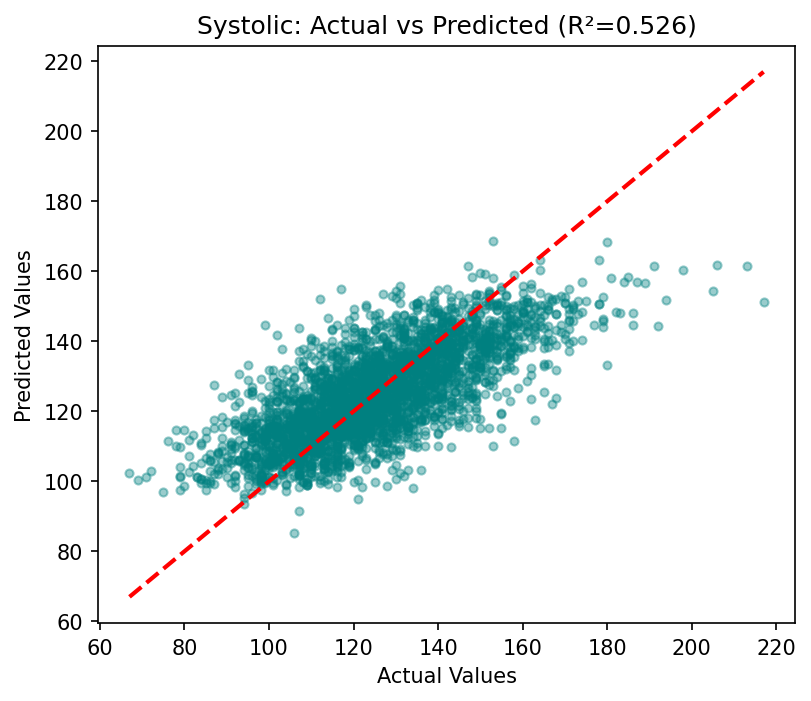
\includegraphics[width=0.48\textwidth]{../presentation/figures/bp_sys_prediction_fig.png}
    \hspace{0.01\textwidth}
    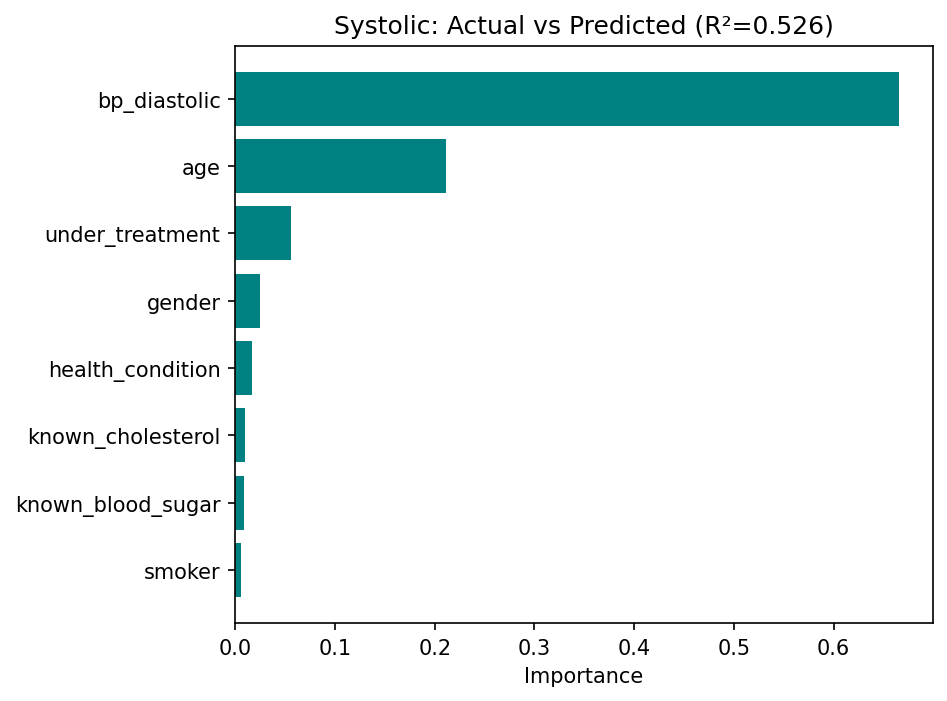
\includegraphics[width=0.48\textwidth]{../presentation/figures/bp_sys_featimp_fig.png}

    \vspace{0.3cm}
    {
    \setbeamercolor{item}{fg=tugreen}
    \begin{itemize}
        \item R² = 0.526, MAE = 10.31 mmHg, RMSE = 13.18 mmHg
        \item \textbf{Diastolic BP} dominates as the strongest predictor (0.67)
        \item Age follows as second most important feature (0.21)
    \end{itemize}
    }
\end{frame}

%==================== HYPOTHESIS 1 ====================
\begin{frame}{}
    \vspace{0.5cm}
    {\raggedright
        {\fontsize{16}{20}\selectfont \color{tugreen} Hypothesis 1 — Age vs Blood Pressure}
    }
    \vspace{0.5cm}
    {
    \setbeamercolor{item}{fg=tugreen}
    \begin{itemize}
        \item H1: Can we statistically prove the relationship between age and BP?
        \begin{itemize}
            % \item Age is the most important predictor for both Systolic and Diastolic BP
            \item Feature importance: Age = 0.673
        \end{itemize}
    \end{itemize}
    }
    \vspace{0.3cm}
    \centering
    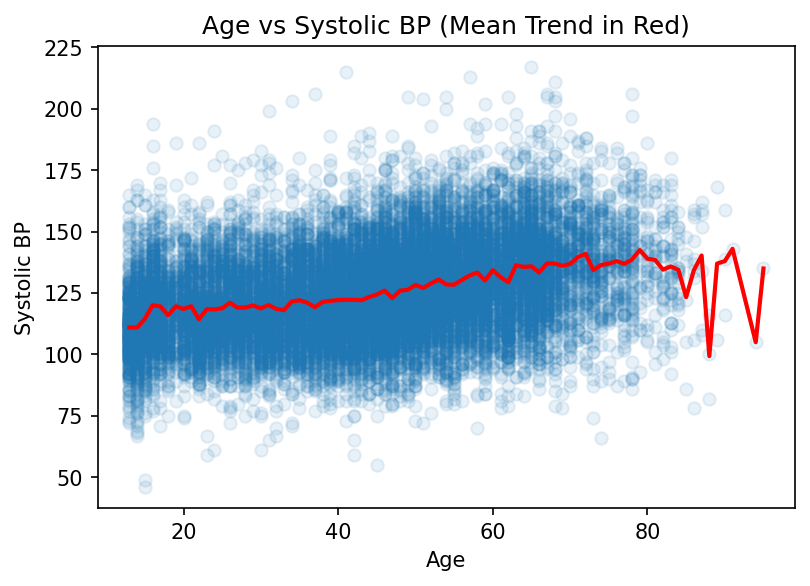
\includegraphics[width=0.65\textwidth, height=0.45\textwidth]{../presentation/figures/bp_vs_age_fig.png}
\end{frame}

%==================== HYPOTHESIS 2 ====================
\begin{frame}{}
    \vspace{0.5cm}
    {\raggedright
        {\fontsize{16}{20}\selectfont \color{tugreen} Hypothesis 2 — Other Factors vs Blood Pressure}
    }
    \vspace{0.5cm}
    {
    \setbeamercolor{item}{fg=tugreen}
    \begin{itemize}
        \item H2: Are there differences in BP by gender, diabetes, smoking, cholesterol, well-being?
        \begin{itemize}
            \item Under Treatment: 0.123 — highest among lifestyle factors
            \item Gender: 0.083
            \item Health Condition: 0.053
            \item Known Blood Sugar: 0.025
            \item Known Cholesterol: 0.024
            \item Smoker: 0.018 — least influential
        \end{itemize}
        \item All factors show \textbf{low importance} compared to Age
        \item R² very low — model cannot distinguish meaningful BP differences by these factors alone
    \end{itemize}
    }
\end{frame}